% !TEX root = jbsilvaThesis.tex

\chapter{\label{chp:nuc_details}Critical Phenomena and Phase Transitions in the Ising Model}

\section{The Ising Model}
The Ising model has been an important model in the study of phase transitions. This model has been used to explain the ferromagnetic transition, financial market  behavior~\cite{geraskin}, and image restoration by computer scientists~\cite{cohen13}. The strength of the Ising model is in its simplicity. The model is constructed by a lattice occupied by spins with a binary set of values at each site typically given by $+1$ and $-1$. The spins interact with each other. In the ferromagnetic case the spins seek to obtain the same value. The anti-ferromagnetic variant of the Ising model has spins which minimize their energy when they have opposing values. The Hamiltonian for the Ising model is given by%%
\begin{equation}
 \label{eq:ising}
	H = -\sum_{{{<}}i,j{{{>}}}} J_{i,j} s_i s_j - h \sum_i s_i
\end{equation}%%
%%
In Eqn.~\eqref{eq:ising} the value of the spin at lattice site $i$ is $s_i$. The field is given by $h$ and the interaction strength between spins $i$ and $j$ is $J_{ij}$.
  
\subsection{Mean-field theory}
The Ising model exhibits a phase transition at a nonzero critical temperature. Mean-field theory calculates  the transition temperature by imposing a self-consistency condition. In  \mf\ theory the interactions with a spin are given relative to their mean value $m$ such that $s_i = m+\delta s_i$. The Ising Hamiltonian can be written as %%
%%
\begin{equation}
	\label{eq:ising2}
	H = -\sum_{{<}i,j{{>}}} J_{i,j} (m+\delta s_i) (m+\delta s_j) - h \sum_i s_i 
\end{equation}%%
%%
By dropping constants and second-order fluctuations $(\delta s)^2$, the Hamiltonian can be simplified as
%%
\begin{equation}
	\label{eq:ising2_2}
	H = -\sum_{i} (Jmz+h)  s_i,
\end{equation}%%
where $z$ is the number of nearest neighbors and we have taken $J_{i,j}=J$ for all $i$ and $j$. The partition function can be easily calculated in this approximation where the spins are uncoupled. The mean value of the magnetization is given by
%%
\begin{equation}
	\label{eq:ising3}
	{<}s{{>}} = m = \tanh \beta(Jmz+h) 
\end{equation}%%
%%
Expanding the hyperbolic tangent function allows us to calculate the critical temperature $T_c$ by imposing the self-consistency condition.%% 
%%
\begin{equation}
	\label{eq:isingtc}
	\beta Jz = 1 \Rightarrow T_c = Jz  
\end{equation}%%
%%
Similarly we obtain the critical exponent for the susceptibility ($\gamma=1$) and the magnetization ($\beta=1/2$).%%
%%
\begin{figure}[!h]
	\centering
	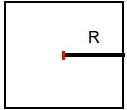
\includegraphics[width=0.35\textwidth]{Images/interbox.png}
	\captionof{figure}{The shape of the interaction with range $R$.}
	\label{fig:interaction}
\end{figure}%%
%%

The simplest interaction is nearest-neighbor, where a given spin interacts with two sites in one dimension and four spins in two dimension for a square lattice. Long-range interactions will be the focus in this dissertation. This interaction is useful because it provides the ability to study long term interaction effects; is convenient, and computationally fast to implement. For ferromagnetic interactions ($J>0$) the effect of the shape of the interaction  does not affect the qualitative nature of the physics. In the anti-ferromagnetic regime ($J<0$) repulsive interactions, geometric frustration, and finite size effects result in a more crucial role of the shape of the interaction.

\section{Landau-Ginzburg Model}
In this section \mf\ theory is reformulated for a \lr\ interaction in a simplified coarse grained model of the Ising model. The coarse graining process takes groups of spins and defines a coarse grained variable which substitutes for this group of spins. The choice of coarse grained variable will be the average magnetization of a hyper-cubic block of spins of length $b$. %%
%%
\begin{equation}
	\label{eq:coarse_graining}
	\phi(r) = \frac{1}{b^d} \sum s_i
\end{equation}%%
%%
To describe the physics under this coarse graining the behavior of the Hamiltonian under this coarse grained procedure must be understood. The most general Hamiltonian includes all powers of the coarse grained variable and its derivatives.%%
%%
\begin{equation}
	\label{eq:hamilt_gen}
H = H(\phi,\partial_u \phi, \partial_u \partial_v \phi,\phi_u \phi_v \ldots) 
\end{equation}%%
%%
From Eqn.~\eqref{eq:ising} one observes that the Hamiltonian is invariant under a sign transformation of both the spin variables at zero field so that the Hamiltonian for the coarse grained variable must obey the following relation.%%
%%
\begin{equation}
	\label{eq:hamilt_gen0}
H(\phi(r),0) = H(-\phi(r),0) 
\end{equation}%%
%%
Under this constraint any odd power terms in the Hamiltonian can be discarded as well as derivatives with similar powers for the coarse grained variables. %%
%%
\begin{equation}
	\label{eq:hamilt_gen1}
H = H( \phi^2, \phi^4, \partial_u \phi_u \partial_v \phi_v, \ldots)
\end{equation}%%
%%
\begin{figure}[!h]
	\centering
	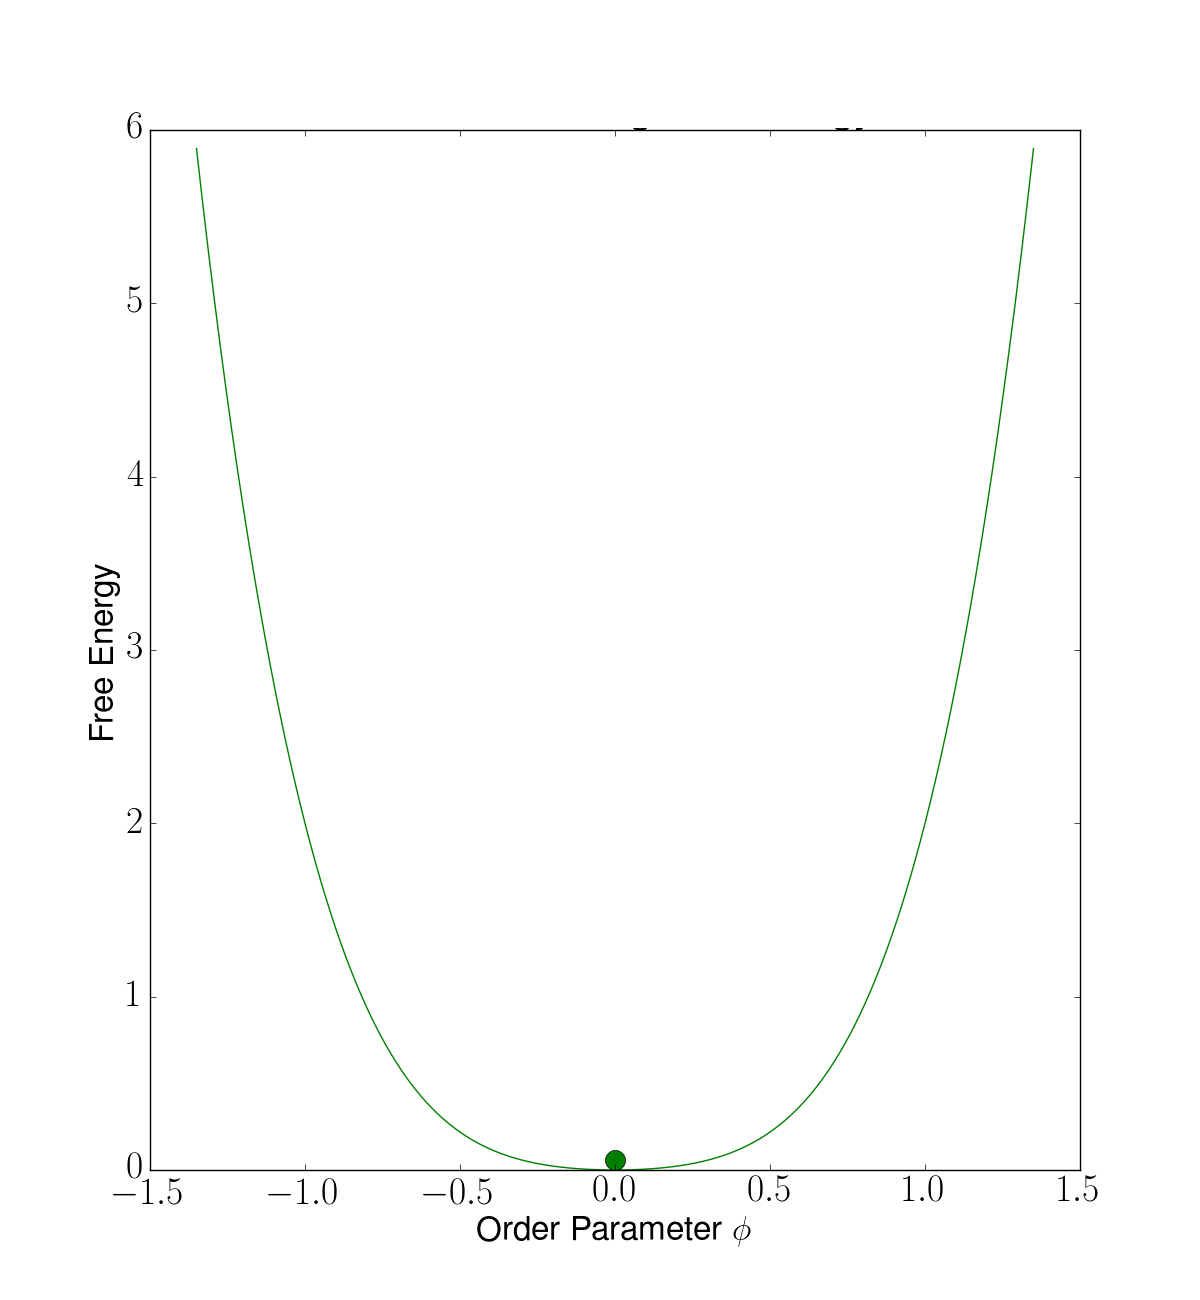
\includegraphics[width=0.6\textwidth]{Images/Classical.png}
	\captionof{figure}{Landau-Ginzburg free energy for $\epsilon > 0$, $h=0$ displaying a single minima.}
	\label{fig:lg-pos}
\end{figure}%%
%%%%
%%%%
%%
\begin{figure}[!h]
	\centering
	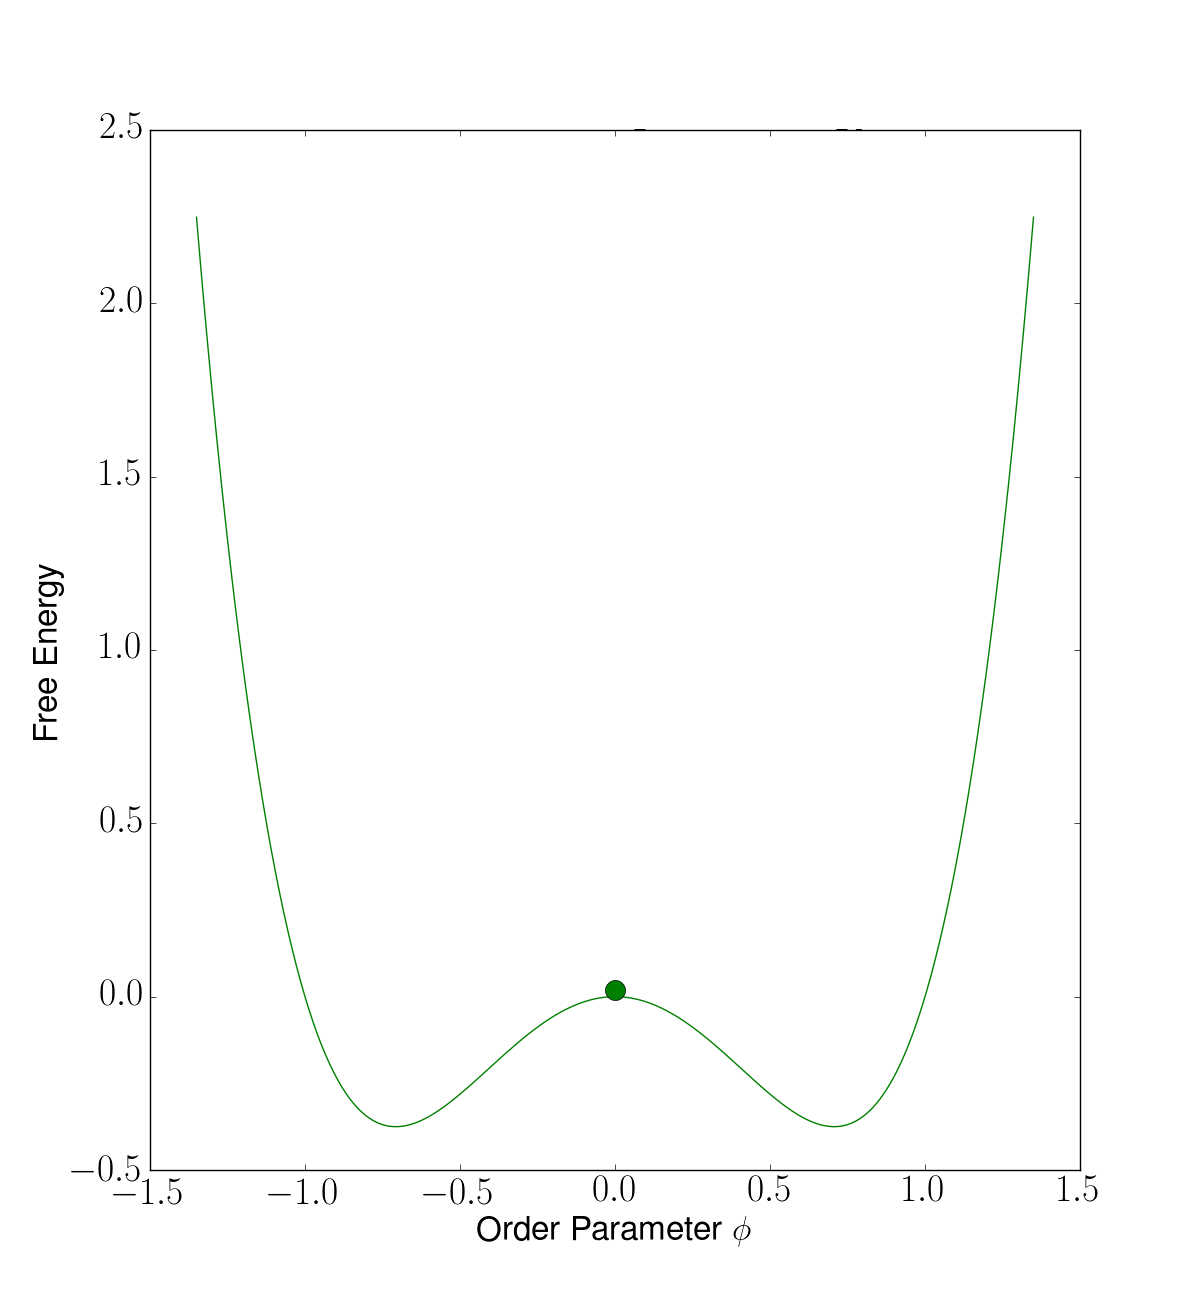
\includegraphics[width=0.6\textwidth]{Images/ClassicalBroken.png}
	\captionof{figure}{Landau-Ginzburg free energy for $\epsilon < 0$, $h=0$ displaying two symmetrical free energy minima.}
	\label{fig:lg-neg}
\end{figure}%%
%%
Dropping higher order terms than $\phi^4$, neglecting derivates higher than second order, and adding a field term leads to the familiar Landau-Ginzburg form with $\epsilon=\frac{T-T_c}{T_c}$.%%
%%
\begin{equation}
\label{eq:landu-ginz_NN}
H = \!\int d^dr (\nabla \phi(r))^2 + \epsilon \phi(r)^2 + \phi(r)^4 -h \phi(r)
\end{equation}%%
%%
This form can alternatively and more rigorously be derived using the Hubbard-Stratonovich transformation~\cite{altland}, from the free energy of the system in contact with a heat bath and Stirling's approximation, or following Ma's derivation~\cite{ma}.
Similarly for a \lr\ interaction of range $R$ the following Landau-Ginzburg Hamiltonian is obtained.%%
%%
\begin{equation}
\label{eq:landu-ginz_R}
H = \!\int d^dr [R^2(\nabla \phi(r))^2 + \epsilon \phi(r)^2 + \phi(r)^4 -h \phi(r) ]
\end{equation}%%
%%
One of the strengths of Landau-Ginzburg theory is how easily spontaneous symmetry breaking is observed when the field  $h$ is zero. In Fig.~\ref{fig:lg-pos} one observes a single minima when $\epsilon > 0$  corresponding to the high temperature disordered state. In contrast, the free energy  for $\epsilon < 0$  has two minima corresponding to  ordered states where the system is dominated by one of the  values of the spin. These results imply a phase transition at $\epsilon = 0$.
%%
\begin{figure}[!h]
	\centering
	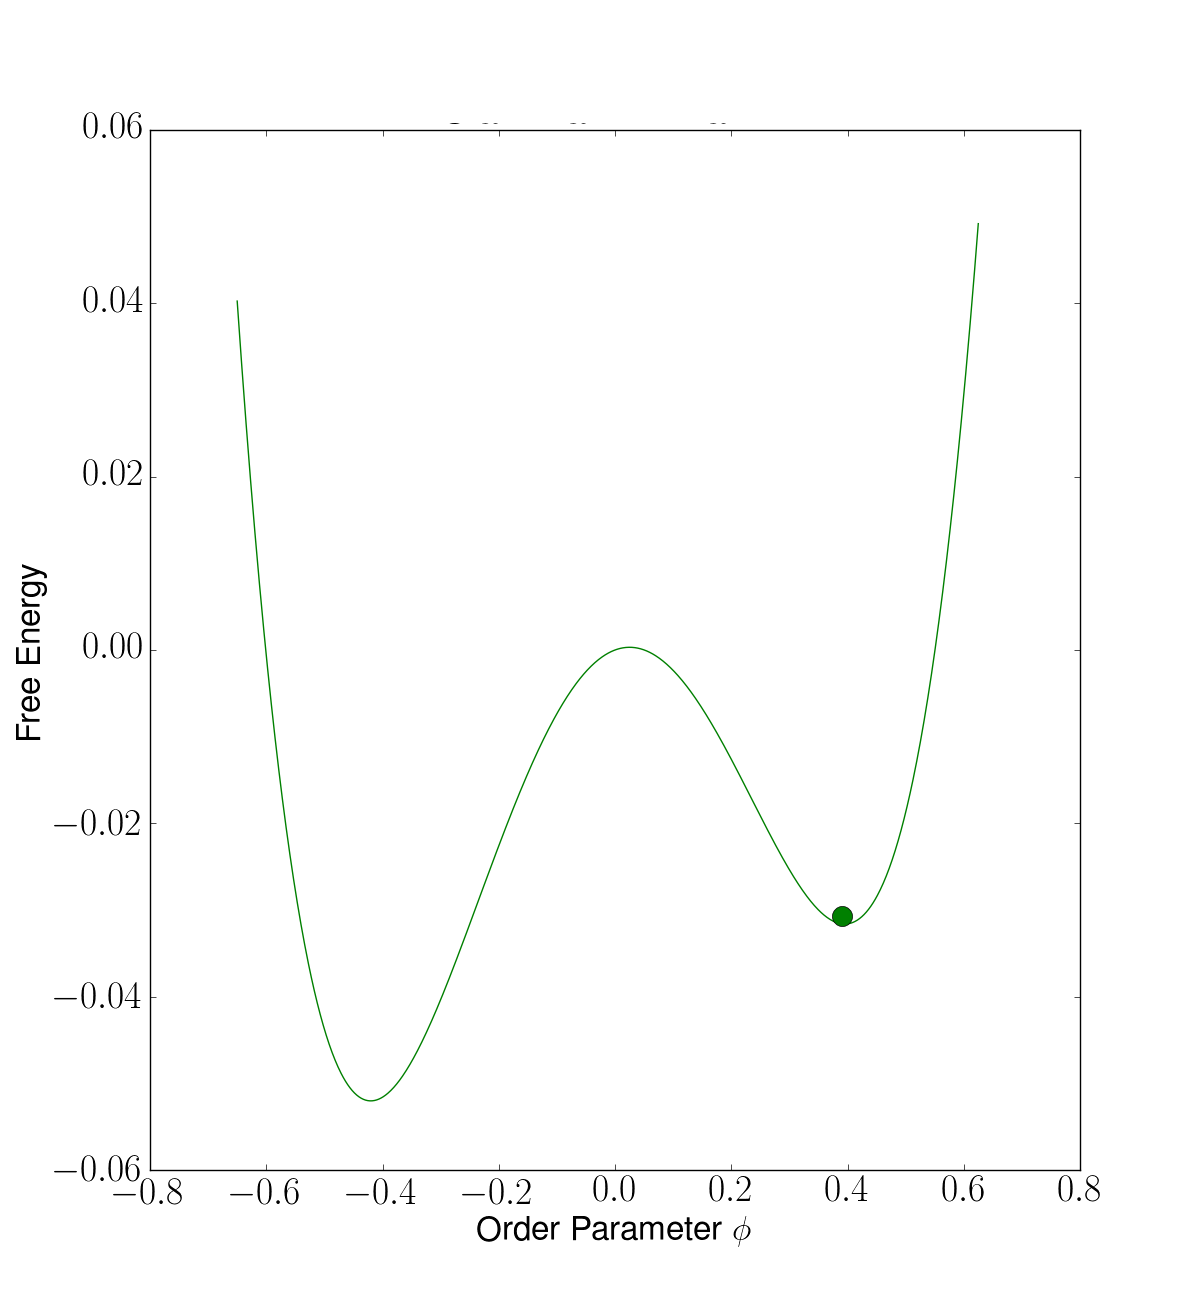
\includegraphics[width=0.6\textwidth]{Images/classicalNucleationStart.png}
	\captionof{figure}{ Landau-Ginzburg free energy with $\epsilon > 0$, $h>0$ displaying a metastable minima and a stable minima. The system sits at the metastable minima.}
	\label{fig:nuc_start_lg}
\end{figure}%%
%%
%%
%%
\begin{figure}[!h]
	\centering
	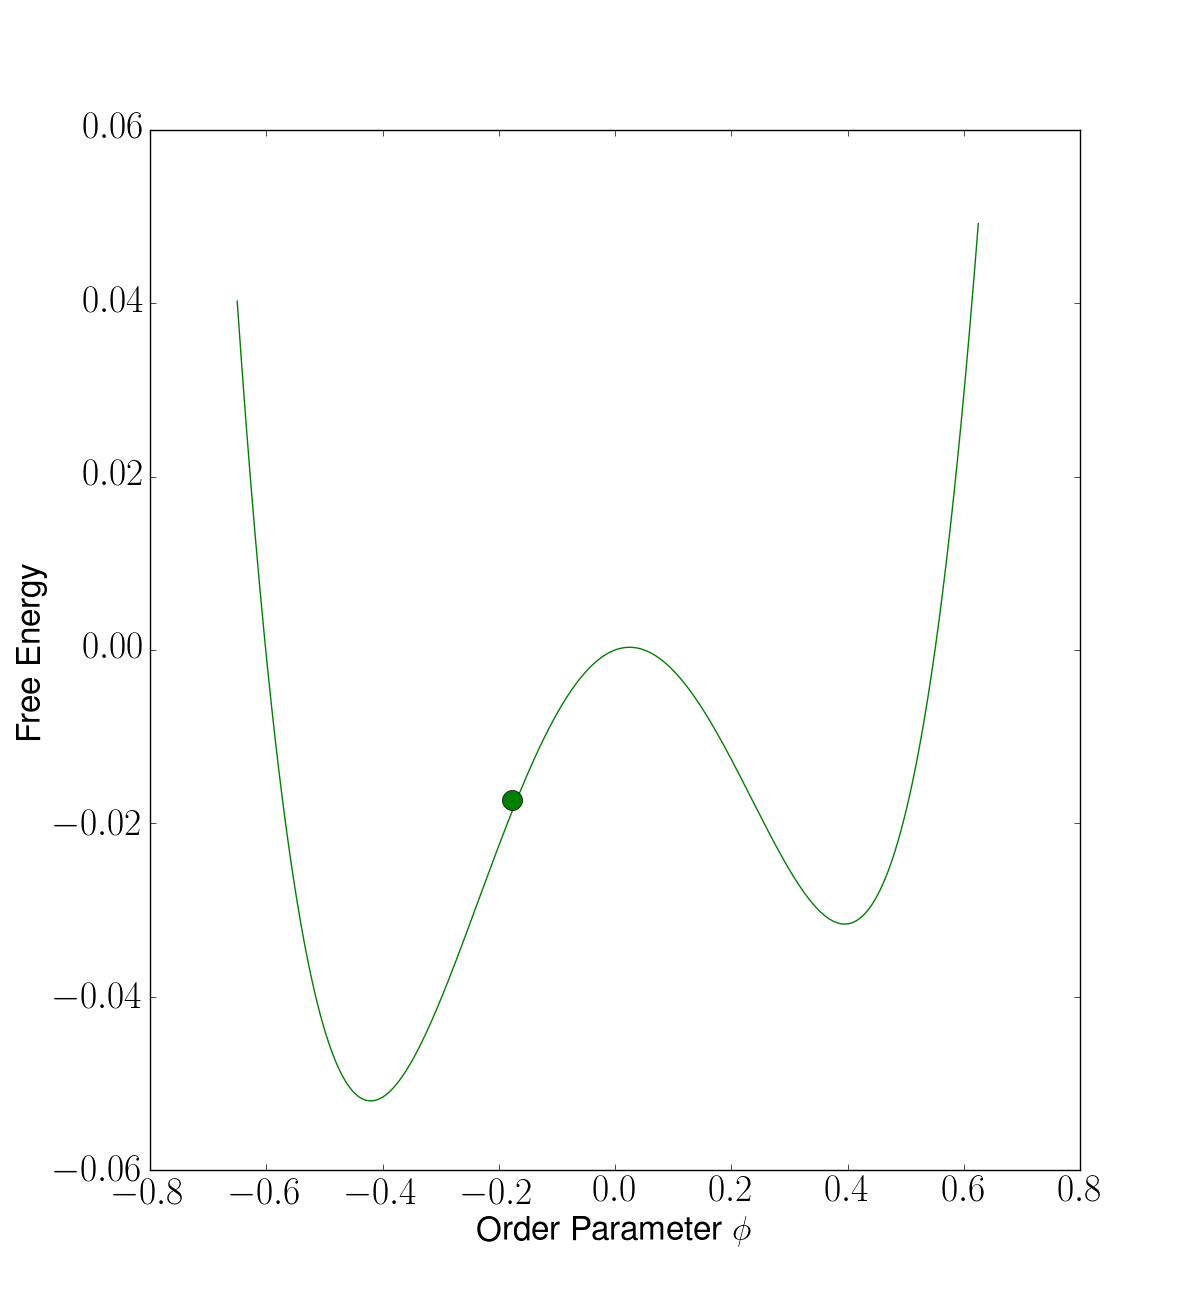
\includegraphics[width=0.6\textwidth]{Images/classicalNucleationHilltop2.png}
	\captionof{figure}{ Landau-Ginzburg free energy with $\epsilon < 0$, $h>0$ displaying a metastable minimum and a stable minimum. The system has traversed the nucleation barrier. }
	\label{fig:nuc_mid_lg}
\end{figure}%%
%%
%%
%%
\begin{figure}[!h]
	\centering
	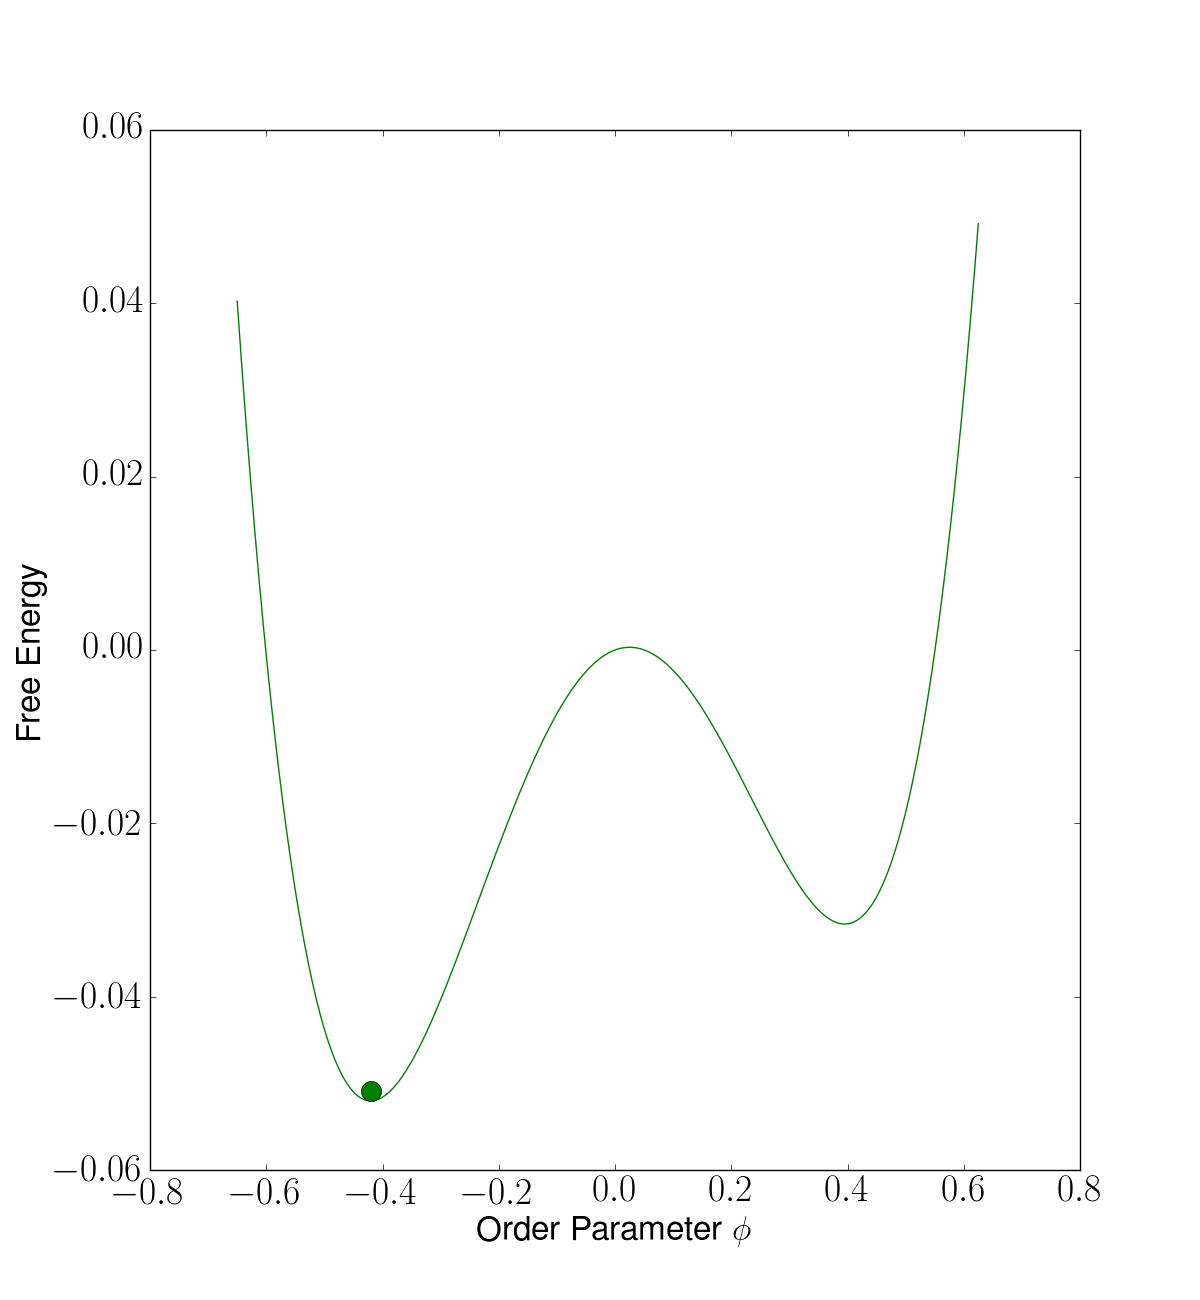
\includegraphics[width=0.6\textwidth]{Images/classicalNucleationEnd.png}
	\captionof{figure}{Landau-Ginzburg free energy with $\epsilon < 0$, $h>0$ displaying a metastable minimum and a stable minimum. System sits at the stable minimum. }
	\label{fig:nuc_end_lg}
\end{figure}%%
%%
By introducing a small nonzero field it is possible to understand nucleation in the Landau-Ginzburg model. In Fig.~\ref{fig:nuc_start_lg} one observes that the small field has changed the relative heights of the minima such that one minimum is metastable and the other minimum is stable. Nucleation in this free energy perspective is the process by which a system that is temporarily trapped in a local minimum reaches the global minimum through energy fluctuations in as shown in Figs.~\ref{fig:nuc_mid_lg} and \ref{fig:nuc_end_lg}. The free energy barrier that the system  must cross is commonly referred to as the nucleation barrier. Intuitively, as the free energy barrier is raised the rate of nucleation is decreased. 

\section{Heterogeneous Ising Model}
Incorporating heterogeneity into the Ising model allows for the modeling more realistic scenarios because most nucleation in the real world originates from \het\ nucleation. 
Heterogeneous nucleation is the process in which the critical droplet forms on a heterogeneity such as a defect, aerosol, or dirt. In this dissertation \het\ nucleation of a single type will be modeled. In this type of \het\ nucleation the magnetization of the spin at a \het\ site will be fixed. The Hamiltonian can then be modified by the introduction of the variable $\epsilon_i$, whose binary value takes on the value $1$ if the spins is fixed or $0$ if dynamic, and the variable $\alpha_i$ which encodes the value of the fixed spin  at the site.%%
%%
\begin{equation}
\label{eq:heter_ising}
H_{\rm impurities} = -\sum\limits_{{<}i,j{>}} J_{i,j} (\epsilon_i (s_i-\alpha_i)+\alpha_i) \epsilon_j s_j -\sum\limits_{i} h (\epsilon_i (s_i-\alpha_i)+\alpha_i) 
\end{equation}%%
%%
\section{Monte Carlo Simulation}
Monte Carlo techniques have proven very useful in sampling such probability distributions. In this work the Metropolis-Hastings algorithm was used to simulate the Ising model.
The Metropolis-Hastings algorithm allows one to sample a probability distribution $P(x)$ given a function $f(x)$ which is proportional to the probability distribution. This condition is highly suggestive of choosing the Boltzmann factor $\exp{(-\beta E)}$ for the function $f(x)$ due to the fact that the probability distribution of a system in thermal equilibrium given by
%%
\begin{equation}
	\label{eq:boltz}
P(E)  = \frac{ \exp{(-\beta E)} }{Z}
\end{equation}%%
%%
One of the conditions for the Metropolis algorithm is that a transition from a state $x$ to a state $y$ must be as likely as the transition from $y$ to $x$. This condition corresponds to  detailed balance. The Metropolis-Hastings algorithm can be summarized by three steps.

\begin{enumerate}
	\item Generate a trial step into a new state from an arbitrary distribution satisfying detailed balance.
	\item Calculate the acceptance probability $\alpha = \frac{f(x_{\rm new})}{f(x_{\rm old})}$. For a system under equilibrium $\alpha = \exp{(-\beta \Delta E )}$.
	
	\item If $\alpha \geq 1$, accept the trial change; otherwise, accept the change with probability $\alpha$; $\alpha \geq 1$ if $\Delta E \leq 0 $.
\end{enumerate} %%
%%
Alternative simulation techniques were also explored including cluster Monte Carlo techniques~\cite{wolff89}, which will be described in later sections as well the Wang-Landau algorithm~\cite{wang01}, which allows for estimation of the density of states.
 
\section{The Intervention Method}
One of the advantages of the intervention method to study nucleation is the ease in which it can be understood from a free energy perspective. In Fig.~\ref{fig:nuc_mid_lg} the system is at a saddle point of the free energy and has formed a critical droplet. At the saddle point the critical droplet can evolve back to the metastable state or to the stable state with equal probability. Therefore, the system at the time of the formation of a critical droplet will evolve into either state with equal probability under a random perturbation. The intervention method is implemented by creating $N$ copies of the system at a time close to when nucleation is expected to occur and allowing the copies to evolve after introducing a perturbation. This perturbation in a copy is commonly introduced by changing the random number generator seed. The nucleation time and location is estimated as the time and location where half of the $N$ copies undergo nucleation at roughly the same time and place as the original droplet.

In this work it will be shown that intervention not only can provide insights into the nucleation process but into the interactions governing the nucleation process.%%
%%
\begin{figure}[!h]
      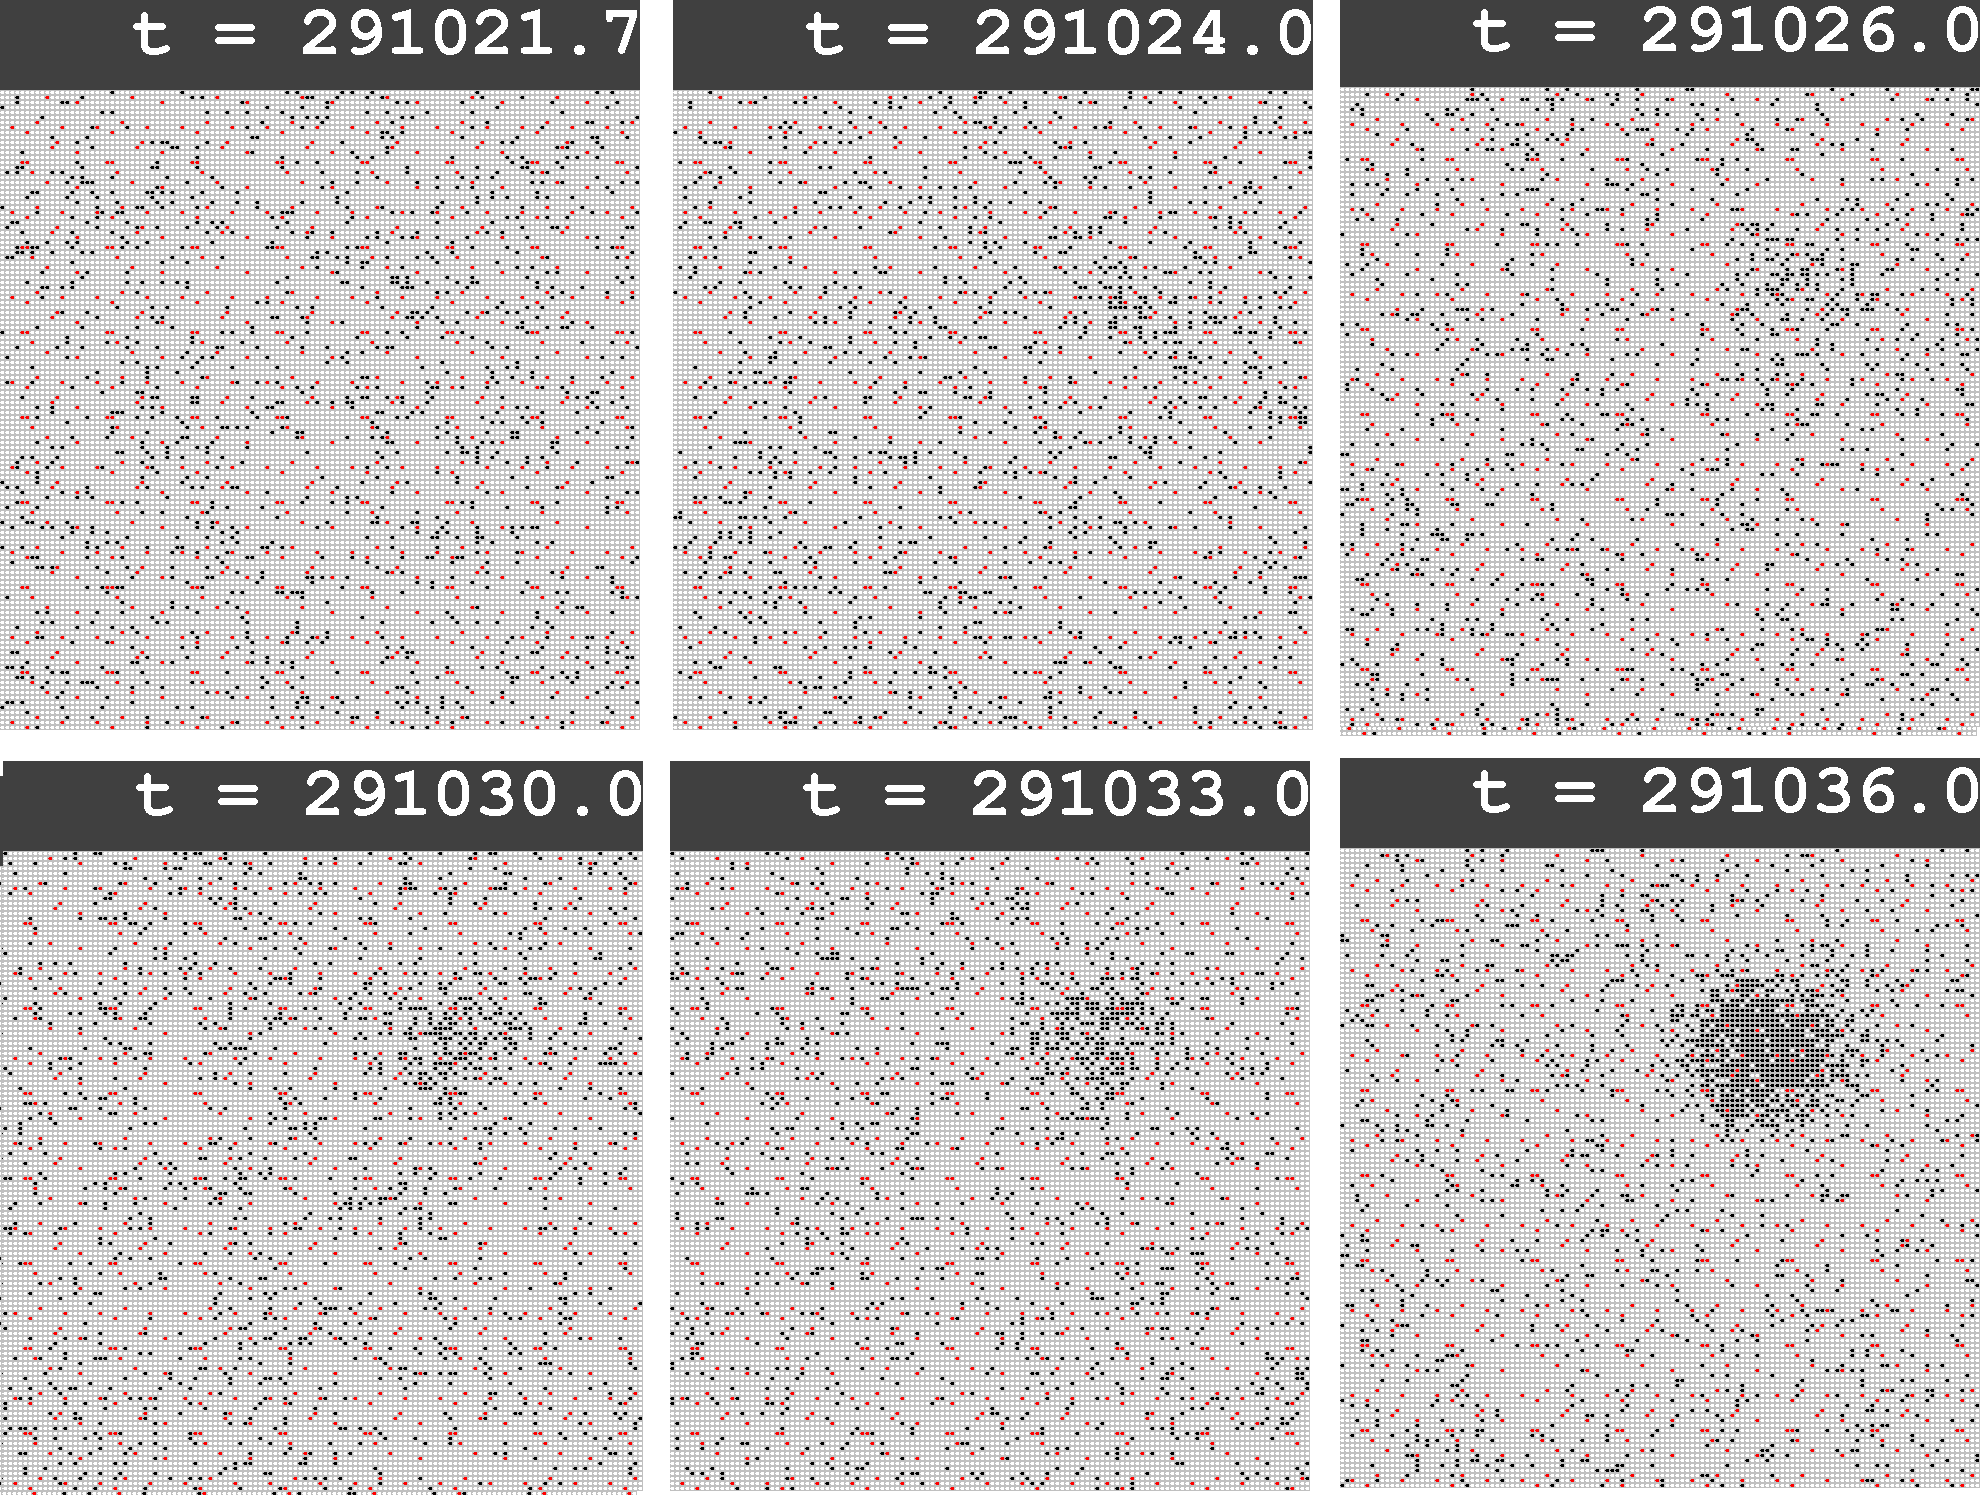
\includegraphics[scale=0.20]{Images/IsingSequence.png}
    \caption{An example of  a sparse nucleating droplet in the \lr\ Ising model with $L=128$, $R=8$, $h=1.0$, $T=1.8$, and $5\%$ non-magnetic  sites placed at random.}
  \label{fig:sequence}
\end{figure}%%
%%
\section{Models of Nucleation}

\subsection{The classical droplet model}

In the classical theory of nucleation a dense droplet is formed by growth from the surface. Aggregation processes can be modeled using a master equation approach. For clusters of size $s$ the cluster can either become smaller or bigger. Assuming a growth rate of $R$ and decay rate of $R'$ the following equation describes the dynamics. %%
%%
\begin{equation}
\frac{\partial n_s}{\partial t}  = + R n_{s-1} - R' n_{s} + R' n_{s+1} - R n_s
	\label{eq:nuc_master}
\end{equation}%%
%%
In thermal equilibrium detailed balance is satisfied.
%%
\begin{equation}
	\label{eq:nuc_master0}
R_{s-1} \exp{(-\beta \Delta F_{s-1})} = R'_{s} \exp{(-\beta \Delta F_{s})} 
\end{equation}%%
%%
We can simplify Eqn.~\eqref{eq:nuc_master} by using Eq.~\eqref{eq:nuc_master0} and taking the continuum limit with $\Delta s = 1$.%%
%%
\begin{equation}
\frac{\partial n_s}{\partial t}  = - \frac{\partial J_s}{\partial s} = \frac{\partial}{\partial s} [
R_s(
-\beta  \frac{\partial \Delta F_s }{\partial s} n_s + \frac{\partial n_s}{\partial s} 
)
]
\label{eq:nuc_master_2}
\end{equation}%%
%%
To calculate the nucleation rate an assumption must be made for the rate of condensation $R_s$ in steady state where the left-hand side of Eqn.~\eqref{eq:nuc_master_2} is equal to $0$. The Becker-Doring assumption is that the condensation rate is proportional to the surface area. The critical droplet  occurs at the critical value of the free energy that denotes the top of the free energy barrier. %%
%%
\begin{equation}
J = J_0 \exp{(-\frac{F_c}{k_B T})}
\label{eq:nuc_becker}
\end{equation}%%
%%%%
%%%%
%%
\subsection{Nucleation near the spinodal}
\label{spinodalnuctheory}
The assumptions of the classical droplet picture break down near the spinodal. In particular, the density of the critical droplet becomes sparse near the spinodal, unlike the predictions of the classical droplet model. The theory of nucleation near the spinodal is outlined in Klein et al~\cite{klein07}. 
%%
%%
%% explain clusters and define%%
%%
The spinodal in the Ising model is  defined in the \mf\ limit when the isothermal susceptibility diverges and the magnetization satisfies  Eqn.~\eqref{eqn:meanfieldmag}, which relates the number of neighbors spins $q$, the coupling strength $J$, magnetization $m$, and the field $h$. %%
%%
\begin{equation}
	\chi = (\frac{\partial m}{\partial h})_T
	\label{eqn:spinodalchi}
\end{equation}%%
%%%%
%%%%
%%
\begin{equation}
	m_s = \tanh[\beta(qJ m_s+h_s)]
	\label{eqn:meanfieldmag}
\end{equation}%%
%%%%
%%
%% diverges as spinodal approaches
%%
%%
By solving Eqs.~\eqref{eqn:spinodalchi} and \eqref{eqn:meanfieldmag}, Eqn.~\eqref{eqn:spinodalhs} is obtained for the spinodal field  $h_{\rm sp}$.
%%
\begin{equation}
h_{\rm sp} = \frac{1}{\beta} \cosh^{-1} \sqrt{\beta q J} - qJ  \sqrt{ \frac{\beta q J - 1}{\beta q J} }
\label{eqn:spinodalhs}
\end{equation}%%

Equation~\eqref{eqn:spinodalhs} defines the set of points which define the spinodal. Near this line the classical picture breaks down and the spinodal picture of nucleation becomes applicable. In this case nucleation occurs by the coalescence of clusters~\cite{monette92,klein07} of spins in the stable direction, where the probability of two interacting spins being part of a cluster is given by Eqn.~\eqref{eqn:bondprob}.

Figure~\ref{fig:clusterEx} displays two clusters defined by this probability. This probability of two like sites joining a cluster goes to zero as the nucleation process continues and the stable spins dominate.

\begin{figure}
	\centering
	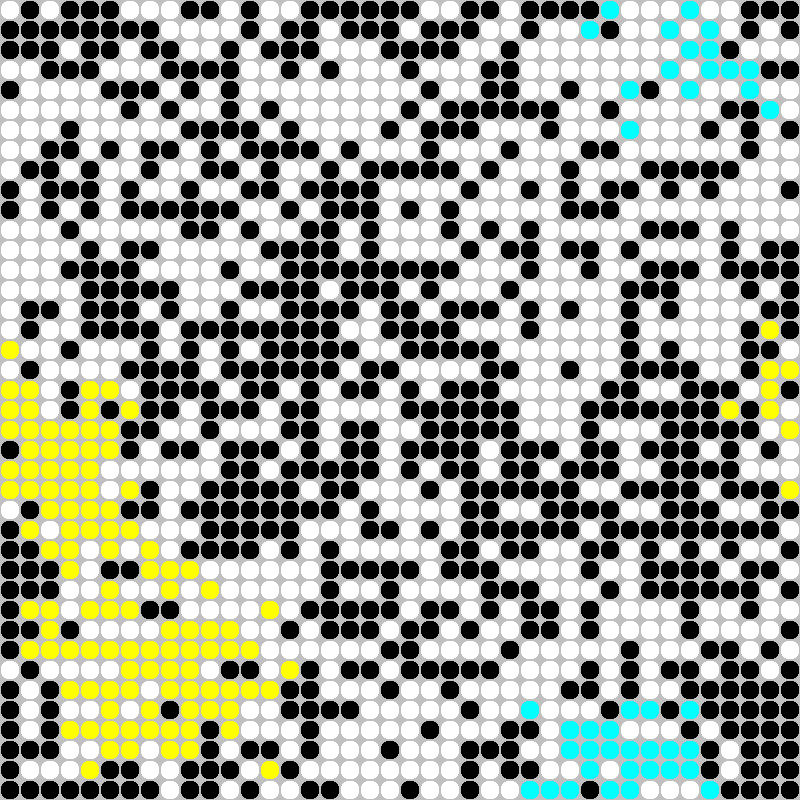
\includegraphics[width=0.6\textwidth]{Images/clusterEx.png}
	\captionof{figure}{ Two large  clusters in a \lr\ Ising model  generated with the bond probability in Eqn.~\eqref{eqn:bondprob}. Yellow denotes the largest cluster.}
	\label{fig:clusterEx}
\end{figure}%%

\begin{figure}[!h]
    \centering
      \includegraphics[scale=1.1]{Figures/intervention_ising/{mean_cluster_in_range_5_per_quilt}.pdf}
    \caption{ The number of  clusters within a correlation length $\xi=11.63$  of the nucleation site in a system with $L=128$, $R=8$, and $T=1.8$. The decrease in the number of clusters is associated with the coalescence process. }
  \label{fig:largeclusternumber}
\end{figure}
%%
%%%%
%%
\begin{equation}
	p_b = 1-\exp{[-\beta J(1-\rho_s)]}
	\label{eqn:bondprob}
\end{equation}%%
%%
%%
%%
The nucleating droplet is a saddle point object which is formed as the clusters coalesce. This coalescence process creates a drop in the total number of percolating clusters as observed in Fig.~\ref{fig:largeclusternumber}. In Fig.~\ref{fig:largeclusternumber} the stable spins in an Ising system are assigned clusters based on the bond probability and the number of clusters is counted within a square box centered at the nucleation site  with a width given by the correlation length. The number of cluster of various sizes is given by Fisher scaling
\begin{equation}
n_s = \frac{\exp{(-\Delta h s^\sigma)}}{s^{\tau-1}}
\label{eqn:fisherscaling}
\end{equation}%%
%%
In Fig.~\ref{fig:mftscaling}  Fisher scaling is observed in Monte Carlo simulations of a near \mf\ \lr\ Ising system. The properties of the  clusters can then be related to the traditional critical exponents $\gamma$ and $\beta$ as defined by Eqs.~\eqref{eqn:tau} and \eqref{eqn:sigma}.   %%
%%%%
%%
\begin{align}
\tau &= 2 + \frac{\beta}{\beta + \gamma}
\label{eqn:tau} \\
\sigma &= \frac{1}{\beta + \gamma}
\label{eqn:sigma}
\end{align}%%

%%
%%
\begin{figure}[!h]
    \centering
      \includegraphics[scale=1.15]{Figures/cluster/{percPure-2}.pdf}
    \caption{ Fisher scaling of cluster sizes for a  \lr\ Ising model with $L=120$, $R=8$, $T=1.8$, and $h=1.14$.}
  \label{fig:mftscaling}
\end{figure}%%
%%
%%
%%
To calculate the nucleation rate we proceed from Eqn.~\eqref{eq:nuc_becker}, which we rewrite in terms of the rate of clusters of size $s$ attaching to the nucleation droplet candidate~\cite{monette92}. This rate is dependent on the availability of clusters of size $s$ and therefore has a proportionally given by Eqn.~\eqref{eqn:spinodalprop} with $\gamma=1$, $\beta=1$, and $\tau=2.5$.%%
%%
%% cluster sizes lead to nucleation behavior
%%
%%
\begin{equation}
	R_s \propto s^{-\frac{3}{2}}
	\label{eqn:spinodalprop}
\end{equation}%%
%%
The nucleation rate obtained from this assumption is given by
%%
\begin{equation}
	J_{\rm sp} \propto \frac{\exp{(-C R^d \Delta h^{\frac{3}{2}-\frac{d}{4}})}}{s^{\frac{3}{2}}}
	\label{eqn:spinodalJ}
\end{equation}%%
%%
Spinodal nucleation theory does not only apply to the \lr\ Ising model, but applies to any system with long-range interactions. There are indications of spinodal nucleation in Lennard-Jones systems~\cite{rashi}.

\section{An Indicator of Spinodal Nucleation }
\label{nonmonoind}

\begin{figure}[!h]
  \centering
      \includegraphics[scale=1.25]{Figures/intervention_ising/{IntervSuccessData-T-1.8-h-1.131-J-1.0-L-160-R-8-4645191778536961024nofit}.pdf}
  \captionof{figure}{ Non-monotonic behavior is observed for a particular trajectory with $L=160$, $R=8$, $h=1.131$, and $T=1.8$. Nucleation is defined as occurring when the intervention success probability first reaches $50\%$. Note that the non-monotonic behavior is preserved as the number of copies is increased.}
  \label{fig:intvnonmono}
\end{figure} %%

\begin{figure}[!h]
  \centering
      \includegraphics[scale=1.25]{Figures/intervention_ising/{IntervSuccessData-T-1.8-h-1.131-J-1.0-L-160-R-8-65520536393690232nofit}.pdf}
  \captionof{figure}{Another nucleation trajectory under the same conditions as Fig.~\ref{fig:intvnonmono} with monotonic behavior. As the number of copies is increased the noise in the success probability decreases. }
  \label{fig:intvmono}
\end{figure} %%
%%
\subsection{Simulation results}

The Ising model can exhibit both classical nucleation and spinodal nucleation given the proper choice of parameters. In this section the flexibility in parameters will be exploited in tandem with the intervention method to explore the role of spinodal nucleation in the occurrence of non-monotonic behavior in the intervention success probability curve as observed in Fig.~\ref{fig:intvnonmono}.

The Metropolis-Hastings algorithm was used to simulate the Ising model. The random number seed for a given nucleation trajectory is recorded to allow for reproduction of a given  nucleation trajectory. After the system is equilibriated an initial high temperature of approximately 50 times the critical temperature the system is quenched to approximately $\frac{4}{9}$ths the critical temperature with a field $\frac{9}{10}$ths the spinodal field limit. The field is then flipped placing the system in a metastable state. The intervention method is then used on the resulting nucleation trajectory by generating runs of $N$ copies of the system at a given intervention time. A random perturbation is then applied by changing the value of the random number seed. The success probability of an intervention is determined by the ratio of runs that are classified as successful to the total numbers of intervention runs. A run is classified as successful if it grows such that one quarter of the system is metastable within $150$ Monte Carlo steps. $150$ Monte Carlo steps is chosen to be much smaller than the average nucleation time for nucleation in Monte Carlo steps hence the unlikelihood of the growth of alternative droplets. The resulting success probability for various intervention times is shown in  Fig.~\ref{fig:intvnonmono} for a random number seed resulting in a trajectory with a non monotonic success probability curve.

The possibility of fluctuations resulting in the observed non-monotonic behavior was first ruled out by increasing the number of intervention runs at a single intervention time. In Figs.~\ref{fig:intvnonmono} and \ref{fig:intvmono} the measurement error for a given intervention time decreases but the larger non-monotonic behavior is maintained only for Fig.~\ref{fig:intvnonmono}. 

The effect of differing properties of the nucleation barriers between spinodal nucleation and classical nucleation could be reflected in the observed behavior. The theory of spinodal nucleation centers around the coalescence of clusters. Given a  spin  configuration we can map this configuration to a collection of clusters using the bond probability.  The statistics of the size of the  clusters can then be used to probe the spinodal nucleation process as the clusters coalesce to form a larger cluster. 

In this spinodal nucleation picture a flat nucleation barrier could result in a trajectory where a nucleating droplet fails to definitively grow in the neighborhood of the nucleation barrier peak. This behavior would be reflected in clusters which fail to coalesce to a single cluster resulting in an inhibited growth in the standard deviation of cluster sizes and the size of the largest cluster. The statistics of percolating clusters for both a non-monotonic trajectory and a monotonic trajectory was measured. This inhibited growth of the largest cluster is displayed in the six Monte Carlo steps after the determined nucleation time in Fig.~\ref{fig:stdcluster} for the green non-monotonic trajectory data for the standard deviation in cluster sizes. %%


By restricting the focus to clusters within an area defined as $1.25R$   from the location of the nucleation droplet Fig.~\ref{fig:stdclusterR} is obtained. It is observed that for the early times right after the onset of nucleation there is a nearly constant behavior in the standard deviation of the cluster sizes occurring near the location of coalescence of the nucleating droplet.  %%
%%%%
%%
\begin{figure}[!h]
    \centering
      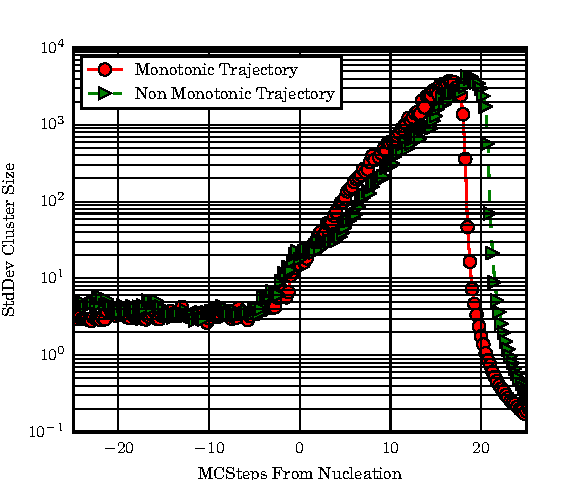
\includegraphics[scale=1.1]{Figures/intervention_ising/stdCluster-.pdf}
    \caption{Standard deviation of the size of all the clusters in the system at times before and after nucleation. The standard deviation increases after nucleation due to the growth of the \nd.}
  \label{fig:stdcluster}
\end{figure}%%
%%%%
%%%%
%%
\begin{figure}[!h]
    \centering
      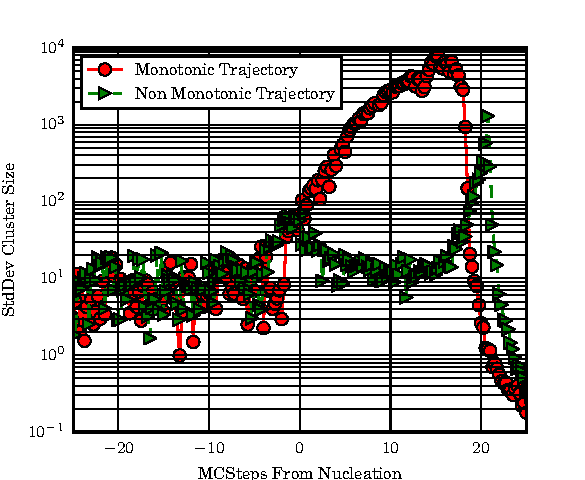
\includegraphics[scale=1.1]{Figures/intervention_ising/stdCluster--inbox-.pdf}
    \caption{ The standard deviation of all clusters within $1.25 R$ of the center of mass of the \nd. The green curve corresponds to a non-monotonic trajectory. My interpretation is that the size of the \nd\ for the non-monotonic trajectory is nearly constant for some time unlike the growth in the monotonic trajectory.}
  \label{fig:stdclusterR}
\end{figure}%%
%%%%
%%
By increasing the interaction range one can  more closely approach the spinodal. If non-monotonic behavior in the nucleating droplet is the result of spinodal nucleation as suggested by the behavior of the clusters, then the number of nucleation trajectories resulting in non-monotonic behavior should increase as a closer approach is made to the spinodal. In Table~\ref{tbl:spinodalnuc} this behavior in the increased likelihood of non-monotonic nucleation trajectories is observed.  %%
%%
\bigskip
\begin{table}[!ht]
\centering
	\begin{tabular}{| l || c | r | c|}
	\hline
Range    & Non-monotonic fraction & Intervention copies & $\Delta h_s$\\
\hline
NN  & 0.0   & 37  & NA      \\
5  & 0.77   & 148 &   0.168 \\
8  & 0.93   & 27 &   0.095 \\
13  & 1.0   & 19  &   0.036 \\ \hline
	\end{tabular}
\caption{The number of non-monotonic trajectories as the spinodal is approached by increasing the interaction range. The percentage  of non-monotonic intervention copies increases as the spinodal is approached.
  	}
\label{tbl:spinodalnuc}
\end{table}%%
%%


\subsection{Nucleation near the spinodal in heterogeneous systems}

In this section the effect of quenched spins on the Ising Hamiltonian will be studied for \lr\ systems. The  Hamiltonian will be rewritten as a random field Ising model where the fixed spins act as an effective field. The central limit theorem will then be used for the case of a uniformly random distribution of fixed spins to show how this effective field in the fully connected Ising model becomes a constant field as expected.   %%
%%
Starting from the \het\  Hamiltonian in Eqn.~\ref{eq:heter_ising} and separating out the fixed spin terms containing $\alpha_i$ from the dynamic terms results in the following equation
%%
\begin{eqnarray}
H_{\rm impurities} = -\sum\limits_{{<}i,j{>}} J_{i,j} \epsilon_i s_i \epsilon_j s_j 
-\sum\limits_{{<}i,j{>}} J_{i,j}  \alpha_j(1-\epsilon_j) \epsilon_i s_i -\sum\limits_{i} h \epsilon_i s_i 
-\sum\limits_{i} h \alpha_i (1-\epsilon_i) 
\end{eqnarray}
.
%%
%%%%
%%
I define a variable $ \mu_i$ for the sum of the fixed spins in the interaction range of the $i$th spin.    %%
%%
\begin{equation}
\mu_i = \sum\limits_{j \in {\rm range}(i)} \alpha_j (1-\epsilon_j) 
\end{equation}%%

By using the definition of $\mu_i$, the \het\ Hamiltonian is given by     %%
%%
%%
%%
\begin{eqnarray}
H_{\rm impurities} = -\sum\limits_{{<}i,j{>}} J_{i,j} \epsilon_i s_i \epsilon_j s_j 
-\sum\limits_{i} J_{i,j}  \mu_i \epsilon_i s_i -\sum\limits_{i} h \epsilon_i s_i 
-\sum\limits_{i} h \alpha_i (1-\epsilon_i) 
\end{eqnarray}
.
%%
%%%%
%%
Combining non-interacting terms in the preceding equation results in %%
%%
%%
%%
\begin{eqnarray}
H_{\rm impurities} = -\sum\limits_{{<}i,j{>}} J_{i,j} \epsilon_i s_i \epsilon_j s_j 
-\sum\limits_{i} (J_{i,j}  \mu_i + h) \epsilon_i s_i 
-\sum\limits_{i} h \alpha_i (1-\epsilon_i) \label{this}
\end{eqnarray} 
.
%%
%%%%
%%
Equation~\eqref{this} can now be expressed   in the form of a random field Ising model  by writing the interaction term as $h_i = (J \mu_i + h)$ and $H_{\rm const} = -\sum\limits_{i} h \alpha_i (1-\epsilon_i) $  %%
%%
%%
\begin{equation}
	\label{eq:heter_w_field}
H_{\rm{impurities\ RFIM}} = -\sum\limits_{{<}i,j{>}} J_{i,j} \epsilon_i s_i \epsilon_j s_j 
-\sum\limits_{i} h_i \epsilon_i s_i 
+H_{\rm constant} .
\end{equation} %%
%%%%
%%
Now suppose the spins are fixed in random locations in the same direction $+1$, such that the fraction of fixed spins to free spins is given by $f_{\rm fixed}$. 
To proceed with the calculation for a range of interaction of any size it is necessary to write $\mu_i$ in a more practical form. This is done by recognizing that $\mu_i$ is given by a binomial distribution such that the expectation value of $\mu_i$ is given by the following if $p = f_{\rm fixed}$.  %%
%%%%
%%
\begin{eqnarray}
{<}\mu_i {>} =  \sum_{k=1}^Q k \binom {Q} {k} p^k (1-p)^{Q-k} \\
{<}\mu_i {>} =  \sum_{k=1}^Q k \binom {Q} {k} f_{\rm fixed}^k (1-f_{\rm fixed})^{Q-k}  = Q f_{\rm fixed}.
\end{eqnarray}%%
%%
From the central limit theorem the stochastic variable $\mu_i$ describing the fixed spin states is approximated by a Gaussian distribution for large values of the range of interaction because it is a sum of identically Bernoulli variables. The central limit theorem also relates the width of the Gaussian to $1/2R+1$
for a square of length $2R+1$. This result agrees with the expected result for a fully connected Ising model. Define the number of spins within range of the interaction by $q$ so that $J= 4/q$. %%
%%%%
%%
\begin{eqnarray}
{<}\mu_i {>} =  f_{\rm fixed} q \\
{<} h_i {>} = 4 \frac{{<} \mu_i{>}}{q} + h \\
h_{\rm eff} = {<} h_i {>} = 4 \frac{q f_{\rm fixed}}{q} + h \\
h_{\rm  eff} =  4 f_{\rm fixed} + h.
\end{eqnarray}%%
The resulting equation describing the effective field is given by 
\begin{equation}
	h_{\rm  eff} =  4 f_{\rm fixed} + h.
	\label{eqn:ran_effect_field}
\end{equation}%%
.
The mean effective field given by Eqn.~\ref{eqn:ran_effect_field} will be of use in describing the result of the uniformly random distributed fixed spins in a single direction in Chapter~\ref{chp:pseudo} as well as understanding the collective behavior of the fixed spins.

\subsection{Introducing and validating \het\ nucleation}

The focus of this section  is on \het\ nucleation, which is defined by a preference for nucleation to occur at specific sites.  The heterogeneity is introduced by fixing the values of spins. The fixed spins can be  introduced by either  randomly dispersing them in the system or introducing a given particular set of spatial correlations. To test the occurrence of \het\ nucleation the sites will be fixed in the stable direction with the location chosen by a uniformly random choice of each of the two-dimensional coordinates.

The Metropolis algorithm was used to simulate nucleation  and the intervention method was used to determine the location of the droplets for each nucleation trajectory. Snapshots of the system at each nucleation event where averaged across the many trajectories to determine the nucleation probability at each location. In Figs.~\ref{fig:fixdensH} and \ref{fig:fixdensProb} the existence of \het\ nucleation is confirmed by the existence of preferential sites for nucleation to occur.   %%
%%
\begin{figure}[!h]
\centering
  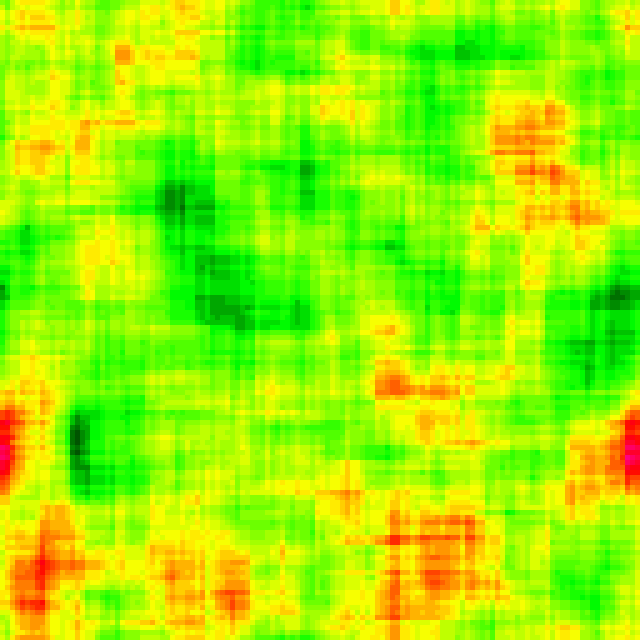
\includegraphics[scale=0.35]{Figures/fix52/Fix52.png}
\captionof{figure}{The density of fixed spins (in the stable direction) within an interaction range of a given site (red corresponds to the highest density and green to the lowest density). The $5.2\%$ fixed spins were inserted at random in an Ising model with $L=120$, $R=8$, and $T=1.8$ (see Figure~\ref{fig:fixdensProb}).}
  \label{fig:fixdensH}
\end{figure}%%

\begin{figure}[!h]
  \centering
      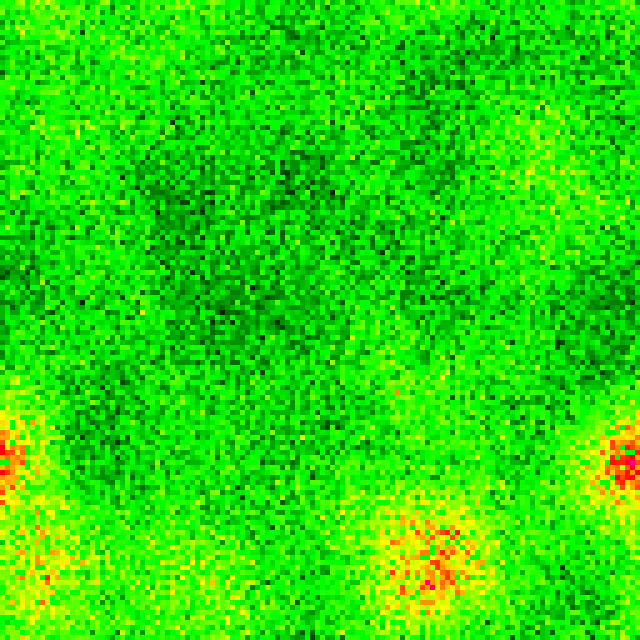
\includegraphics[scale=0.35]{Figures/fix52/ER52.png}
 \captionof{figure}{ The nucleation probability corresponding to the configuration in  Fig.~\ref{fig:fixdensH}. Note that nucleation is more likely to occur at the sites with a higher density of fixed spins.}
  \label{fig:fixdensProb}
\end{figure}%%
%%
To isolate \het\ nucleation effects a disordered quilt-like pattern is introduced that appears nearly \homo\ to an Ising site. This pattern will be referred to as a ``quilt" disorder arrangement. This arrangement is generated by first generating a disorder arrangement of fixed spins in a $(2R+1)$ square. This pattern is then applied across the system in a manner identical to that in the creation of a quilt. If the system length is an integer multiple of $(2R+1)$ this quilt pattern will create a pattern which does not exhibit \het\ nucleation due to effects in the edge of the quilt pattern. In this work two types of disorder will be used; namely, the fixed spin arrangement with an uniformly random choice of coordinates and this quilted fixed spin pattern. The value of the fixed spins will be chosen to be either an equal mix of up and down spins or composed of all up or down spins. 

%%%%%%%%%%%%%%%%%%%%%%%%%%%%%%%%%%%%%%%%%%%%%%%%%%%%%%%%
%%%%%
%%%%%%%%%%%%%%%%%%%%%%%%%%%%%%%%%%%%%%%%%%%%%%%%%%%%%%%%%%%%%%%%%%%%%%%%%%%%%%%%%%%%%%%%%%%%%%%%%%%%%%%%%%%%%%%%
